%%% The ``\documentclass'' command has one parameter, based on the kind of
%%% document you are preparing.
%%%
%%% [annual] - Technical paper accepted for presentation at the ACM SIGGRAPH 
%%%   or SIGGRAPH Asia annual conference.
%%% [sponsored] - Short or full-length technical paper accepted for 
%%%   presentation at an event sponsored by ACM SIGGRAPH
%%%   (but not the annual conference Technical Papers program).
%%% [abstract] - A one-page abstract of your accepted content
%%%   (Technical Sketches, Posters, Emerging Technologies, etc.). 
%%%   Content greater than one page in length should use the "[sponsored]"
%%%   parameter.
%%% [preprint] - A preprint version of your final content.
%%% [review] - A technical paper submitted for review. Includes line
%%%   numbers and anonymization of author and affiliation information.

\documentclass[annual]{acmsiggraph}

%%% If you are submitting your paper to one of our annual conferences - the 
%%% ACM SIGGRAPH conference held in North America, or the SIGGRAPH Asia 
%%% conference held in Southeast Asia - there are several commands you should 
%%% consider using in the preparation of your document.

%%% 1. ``\TOGonlineID''
%%% When you submit your paper for review, please use the ``\TOGonlineID''
%%% command to include the online ID value assigned to your paper by the
%%% submission management system. Replace '45678' with the value you were
%%% assigned.

\TOGonlineid{45678}

%%% 2. ``\TOGvolume'' and ``\TOGnumber''
%%% If you are preparing a preprint of your accepted paper, and your paper
%%% will be published in an issue of the ACM ``Transactions on Graphics''
%%% journal, replace the ``0'' values in the commands below with the correct
%%% volume and number values for that issue - you'll get them before your
%%% final paper is due.

\TOGvolume{0}
\TOGnumber{0}

%%% 3. ``TOGarticleDOI''
%%% The ``TOGarticleDOI'' command accepts the DOI information provided to you
%%% during production, and which makes up the URLs which identifies the ACM
%%% article page and direct PDF link in the ACM Digital Library.
%%% Replace ``1111111.2222222'' with the values you are given.

\TOGarticleDOI{1111111.2222222}

%%% 4. ``\TOGprojectURL'', ``\TOGvideoURL'', ``\TOGdataURL'', ``\TOGcodeURL''
%%% If you would like to include links to personal repositories for auxiliary
%%% material related your research contribution, you may use one or more of
%%% these commands to define an appropriate URL. The ``\TOGlinkslist'' command
%%% found just before the first section of your document will add hyperlinked
%%% icons to your document, in addition to hyperlinked icons which point to
%%% the ACM Digital Library article page and the ACM Digital Library-held PDF.

\TOGprojectURL{}
\TOGvideoURL{}
\TOGdataURL{}
\TOGcodeURL{}

%%% Replace ``PAPER TEMPLATE TITLE'' with the title of your paper or abstract.

\title{PerVERT: The Performance Visualization and Error Remediation Toolkit}

%%% The ``\author{}'' command takes the names and affiliations of each of the
%%% authors of your paper or abstract. The ``\thanks{}'' command takes the
%%% contact information for each author.
%%% For multiple authors, separate each author's information by the ``\and''
%%% command.

\author{Niels Joubert\thanks{e-mail:njoubert@cs.stanford.edu}\\ Stanford University %
\and Eric Schkufza\thanks{e-mail:eschkufz@cs.stanford.edu}\\ Stanford University}

%%% The ``pdfauthor'' command accepts the authors of the work,
%%% comma-delimited, and adds this information to the PDF metadata.

\pdfauthor{Niels Joubert, Eric Schkufza}

%%% Keywords that describe your work. The ``\keywordlist'' command will print
%%% them out.

\keywords{performance visualization, JIT, compiler, instrumentation}

%%% The ``\begin{document}'' command is the start of the document.

%%% If you have user-defined macros, you may include them here.

% example of a user-defined macro called ``remark.''
% \newcommand{\remark}[1]{\textcolor{red}{#1}}

\begin{document}

%%% A ``teaser'' image appears under the title and affiliation information,
%%% horizontally centered, and above the two columns of text. This is OPTIONAL.
%%% If you choose to have a ``teaser'' image, it needs to be placed between
%%% ``\begin{document}'' and ``\maketitle.''

\teaser{
   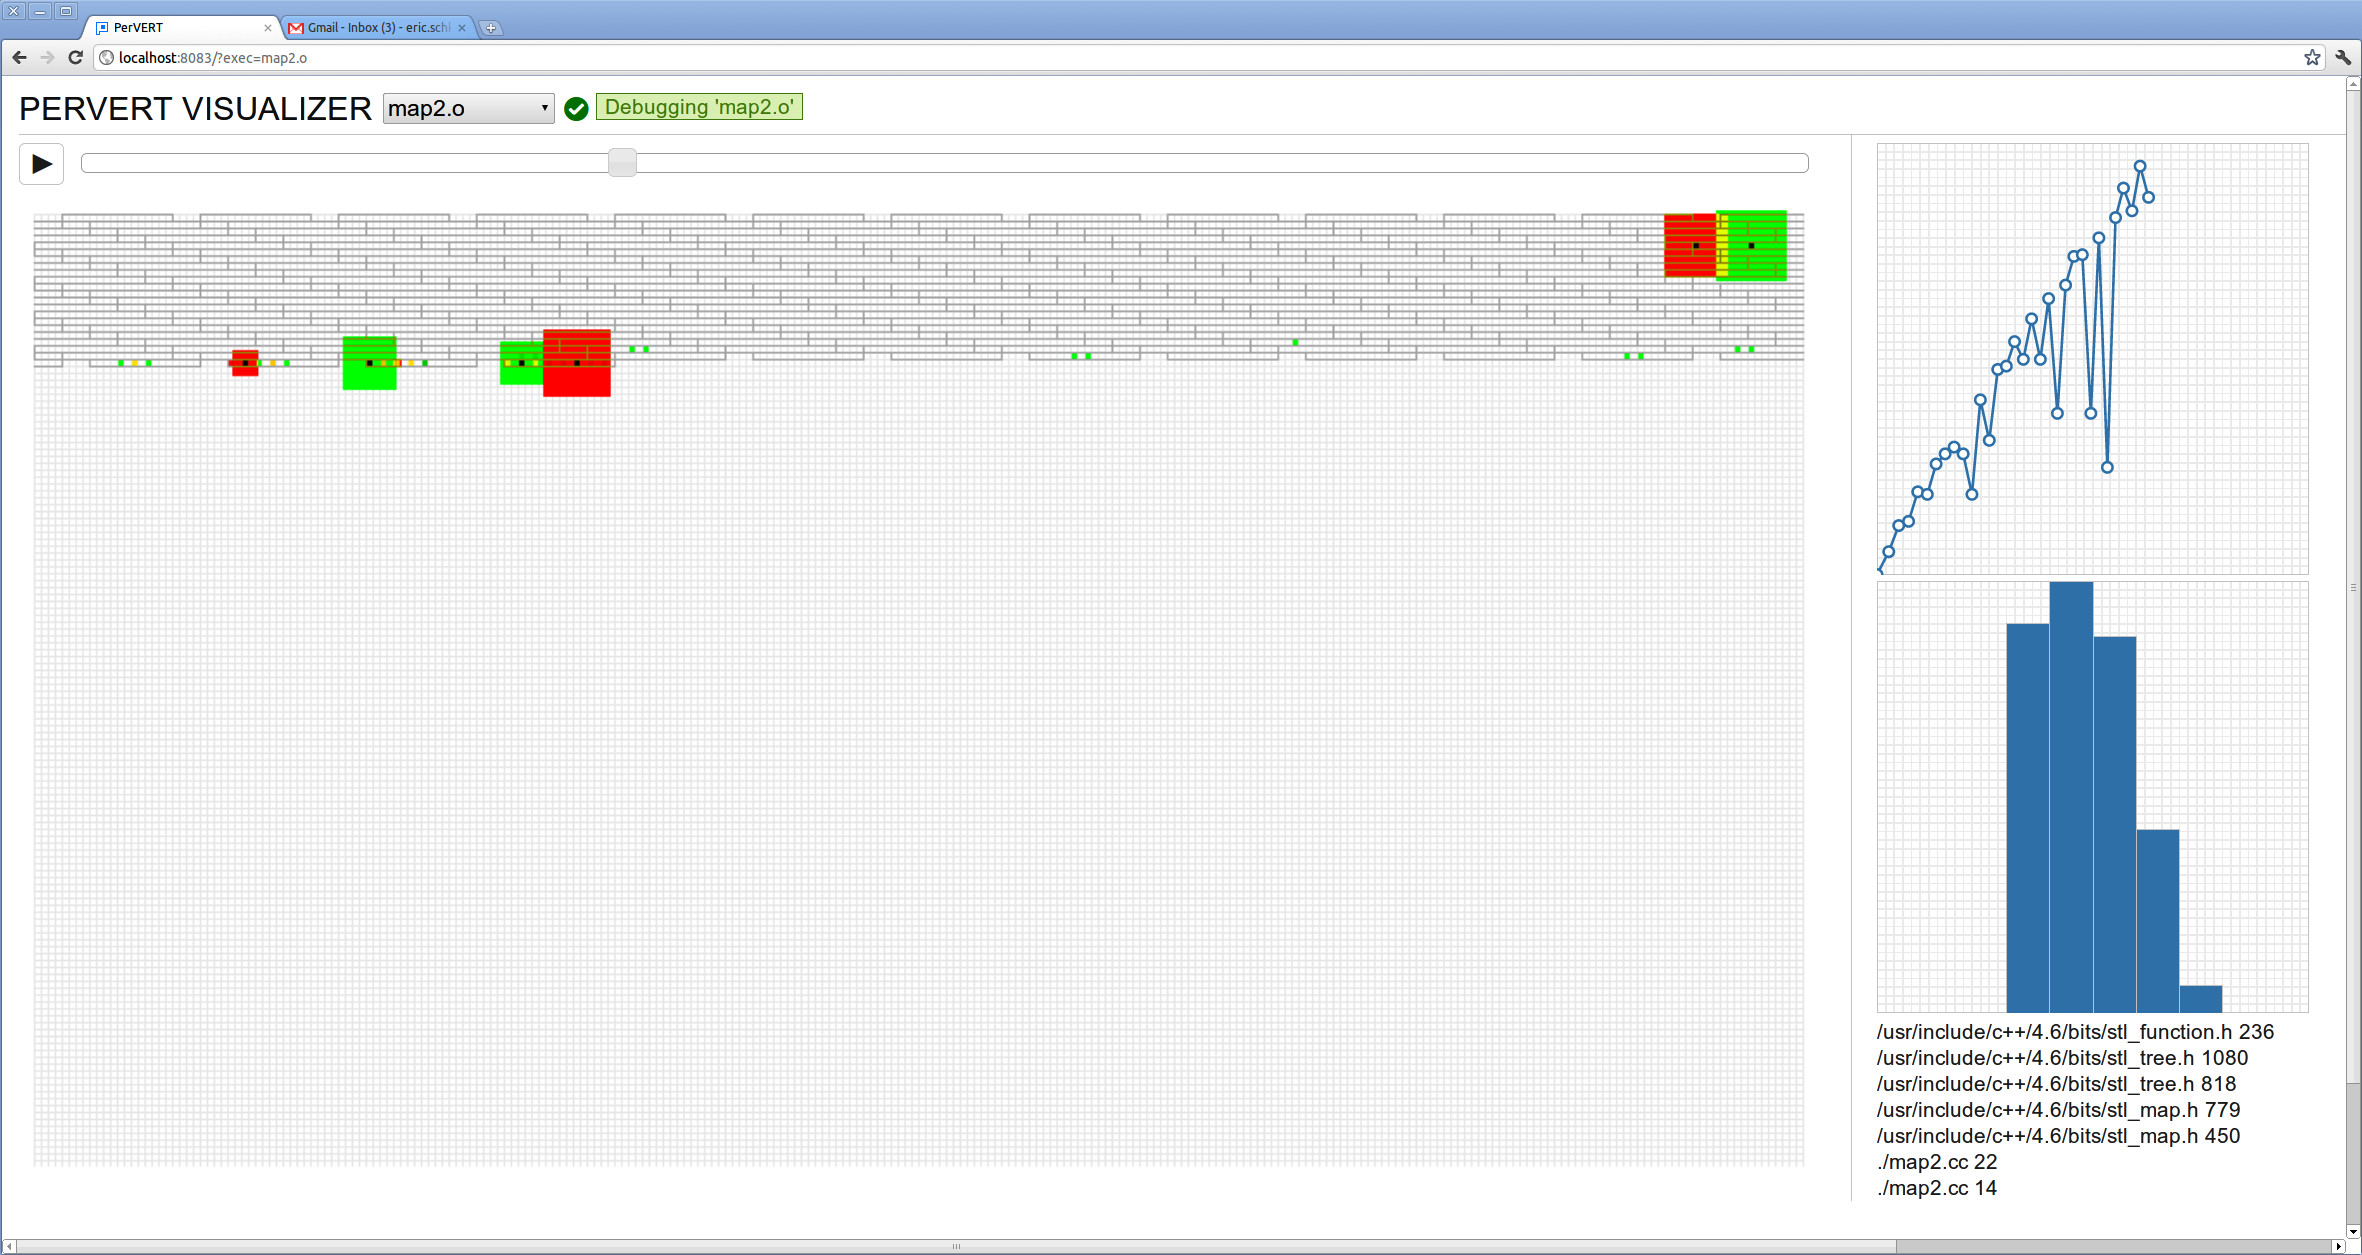
\includegraphics[height=3in]{images/pervert.png}
   \caption{Spring Training 2009, Peoria, AZ.}
}

%%% The ``\maketitle'' command must appear after ``\begin{document}'' and,
%%% if you have one, after the definition of your ``teaser'' image, and
%%% before the first ``\section'' command.

\maketitle

%%% Your paper's abstract goes in its own section.

\begin{abstract}

Performance tuning is an important step in the development large software systems. 
Examples include web-servers which routinely handle thousands of simultaneous content requests, 
  and petaflop supercomputers which perform physical simulations that span tens of thousands of cpu cores. 
As improvements in clock frequency slow and hardware trends continue towards increased parallelism, 
  the runtime performance of these and similar systems will become ever more a function of memory efficiency. 
Unfortunately, the ability to effectively reason about this phenomenon using existing tools such as valgrind, gprof, or gdb, 
  through a text-based interface, is limited, and tedious at best.

We present PerVERT, an instrumentation framework for logging a process's virtual memory traffic and a visualization suite for reasoning about common memory performance bugs: 
  Are memory accesses organized coherently in both spatial and temporal dimensions? 
  To what extent do these patterns differ based on program inputs or changes in source code?
\end{abstract}

%%% ACM Computing Review (CR) categories.
%%% See <http://www.acm.org/class/1998/> for details.
%%% The ``\CRcat'' command takes four arguments.

\begin{CRcatlist}
  \CRcat{I.3.7}{Computer Graphics}{Three-Dimensional Graphics and Realism}{Radiosity};
\end{CRcatlist}

%%% The ``\keywordlist'' command prints out the keywords.

\keywordlist

%%% The ``\TOGlinkslist'' command will insert hyperlinked icon(s) to your
%%% paper. This includes, at a minimum, hyperlinked icons to the ACM article
%%% page and the ACM Digital Library-held PDF. If you added URLs to
%%% ``\TOGprojectURL'' or the other, similar commands, they will be added to
%%% the list of icons.
%%% Note: this functionality only works for annual-conference papers.

\TOGlinkslist

%%% The ``\copyrightspace'' command 
%%% Do not remove this command.

\copyrightspace

%%% This is the first section of the body of your paper.

\section{Introduction}
  Do this last.

\section {Motivation}
  \begin{itemize}
    \item High performance codes need to be as fast as possible. 
    \item Performance is a function of memory efficiency.
    \item
      
  \end{itemize}

\section {Design}

\section {Implementation}
  \begin{itemize}
    \item Often have to do remote performance tuning.
    \item Development environment often divorced from production environment -- examples.
    \item Useful to divorce visualization frontend from analysis and binary instrumentation
    \item Also allows us to leverage existing suite of html visualization tools.
    \item Built up from three parts -- described below
  \end{itemize}

  \subsection{Binary Instrumentation}
    \begin{itemize}
      \item What it is: Pintool plugin
      \item Produces memory trace
      \item Intercept X86 to find read/write instructions
      \item Intercept function calls to find malloc/free
      \item Save as trace file
    \end{itemize}
  \subsection{Backend}
    \begin{itemize}
      \item System is designed to handle massive amounts of data.
      \item Static index built over that data.
      \item On demand analysis done in response to user interaction.
      \item To optimize this, we unify analysis of and interface to data.
    \end{itemize}

    % bo popsicle

    \subsubsection{Index}
      \begin{itemize}
        \item What is is: Persistent long running analysis server
        \item Read and index trace files (what indices?)
        \item Read and index debug symbols from executable (what symbols?)
      \end{itemize}
      
      % eric above
      % june sandwich -- 
      % niels below

    \subsubsection{Server}
      \begin{itemize}
        \item HTTP JSON server
        \item Serves frontend / presents JSON api
        \item Persistently captures all executables so that you can do comparisons between runs.
        \item A stateless api so that multiple users can view the same data or one user can close and come back.
      \end{itemize}

  \subsection{Frontend}
    \begin{itemize}
      \item Web app: user interaction initiates asynchronous request for textual data - then render as visualizations.
      \item Caching layer stores interaction history to minimize backend communication
      \item Use canvas to draw memory space / pixel pushing.
      \item D3 to draw aggregate statistics
    \end{itemize}

\section {Example Applications}
  \subsection{Algorithm}
  \subsection{Variants}
    \begin{itemize}
      \item C++ array
      \item C++ STL vector
      \item C++ STL map
      \item Haskell list
    \end{itemize}

\section {Related Work}

\section{Future Work}
  \subsection{Visualization and Interaction}
  \begin{itemize}
    \item Diffmaps for comparing across revisions
    \item Aggregate views for massive amounts of data
    \item User-defined data filtering
  \end{itemize}

  \subsection{Data Collection and Analysis}
  \begin{itemize}
    \item Physical memory simulator
    \item Supporting incomplete data / sampling
    \item Selective data capture
  \end{itemize}

\section{Conclusion}
  Do this last.

\bibliographystyle{acmsiggraph}
\bibliography{template}
\end{document}
